\documentclass[a4paper,twocolumn,dvipdfm]{article}

% Učitaj pakete za kodnu stranicu utf8 i hrvatski jezik.
\RequirePackage[utf8]{inputenc}
\RequirePackage[croatian]{babel}

% Paket za hrvatski jezik neispravno izostavlja točke iza naslova,
% to ispravljamo zadavanjem novih funkcija za numeriranje koje stavljaju
% točku.
\makeatletter
\renewcommand\thesection{\@arabic\c@section.}
\renewcommand\thesubsection{\thesection\@arabic\c@subsection.}
\renewcommand\thesubsubsection{\thesubsection\@arabic\c@subsubsection.}
\renewcommand\theequation{\@arabic\c@equation}
%\renewcommand\thefigure{\@arabic\c@figure.}
%\renewcommand\thetable{\@arabic\c@table.}
\makeatother

% Ostali korisni paketi.
\RequirePackage{graphicx}
\RequirePackage[unicode]{hyperref}
\RequirePackage{amssymb}
\RequirePackage{amsmath}
\RequirePackage{pstricks}
\RequirePackage{booktabs}
\RequirePackage{multirow}


% Ovdje započinje članak.
\begin{document}

% Navedite naslov i autore. Datume se automatski postavlja na datum kreiranja dokumenta,
% no može se promijeniti zadavanjem \date{30. veljače, 2004.}
\title{Raspoznavanje rukom pisanih slova na ispitnim obrascima} 
\author{Tomislav Grbin, Mihej Komar, Ivan Kravarščan, Toni Pivčević i Ivana Stokić}
\maketitle

% Svako poglavlje započinje sa \section{Ime poglavlja} ako želimo da bude
% numerirano, a sa \section*{Ime poglavlja} ako ne želimo da bude numerirano.

\section*{Sažetak}
U ovom radu je prikazana metoda raspoznavanja dijela tiskanih slova abecede (od
A do J) i znaka crtice unutar polja za ispravak odgovora na ispitnim obrascima.
Opisani su postupci pretprocesiranja slike s ciljem povećanja invarijantnosti na
veličinu, debljinu, intenzitet linija i poziciju. Pokazano je kako se
različitim metodama izlučivanja značajki i klasifikacije znatno povećava stupanj
točnosti klasifikacije. Za klasifikaciju su upotrijebljeni: višeslojni
perceptron, radijalne neuronske mreže i K-najbližih susjeda. Napravljena je
procjena sigurnosti u dobivenu klasifikaciju. Izrađeni sustav ima točnost od
97,45\% bez određivanja sigurnosti klasifikacije i 99,41\% uz 6,92\% nesigurnih
klasifikacija.

\section{Uvod}
Na nekim ispitnim obrascima postoje polja u koje student rukom upisuje željeni
odgovor u obliku jednog slova engleske abecede (slova od A do J) ili crticu ako
je odustao od odgovaranja na pitanje. Tema ovog rada bila je osmišljanje i
implementacija sustava koji prepoznaje napisano slovo. Predviđena je integracija
s već postojećim sustavom za izradu i očitavanje ispitnih obrazaca. Postojeći
sustav bi izdvajao sliku kućice s obrasca te ju predao kao ulaz sustavu
koji bi trebao biti izrađen u okviru ovog projekta. Zbog jednostavnosti
integracije, izrađeni sustav je potpuno izrađen u programskom jeziku Java.

Postojeći sustav već ima mogućnost ručne klasifikacije slova pa je predviđeno
da se ovim sustavom slovo klasificira ako je rezultat visoke vjerojatnosti. Ako
klasificirano slovo nije vjerojatno, klasificiranje se prepušta korisniku. S
obzirom na to da je najveći broj polja prazno, bilo ih je potrebno vrlo brzo
klasificirati.

Sustav je podijeljen na tri osnovna dijela: pretprocesiranje slike, izlučivanje
značajki i klasifikaciju. Dio ideja je dobiven iz \cite{vamvakasoptical}.
Pretprocesiranje slike je potrebno kako bi slika bila u formatu prilagođenom za
izlučivanje značajki i invarijantna na veličinu, debljinu, intenzitet linija i
poziciju slova unutar polja. Izlučivanje značajki je postupak kako neku sliku
predstaviti jednim vektorom i to tako da što su dvije slike sličnije, udaljenost
između dobivenih vektora je manja.

Klasifikacija je postupak strojnog učenja gdje je cilj ulazni vektor pridružiti
određenoj klasi. Kako bi se povećala točnost sustava, izrađeno je više
klasifikatora, a svi dobiveni rezultati su integrirani u jedan glavi rezultat.
Više klasifikatora je postignuto pomoću više različitih metoda izlučivanja
značajki i klasifikatora. Na Slici \ref{figure:cijeliSustav} su prikazane sve
komponente sustava uz opisanu podjelu.

Za prikaz rada pretprocesiranja korišteno je jednostavno grafičko sučelje.
S lijeve strane odabere se direktorij iz kojeg se izvlače sličice. Unutar istog
direktorija su sličice za koje bi rezultat klasifikacije trebao biti isti.
Nakon odabira, s desne strane prikazuju se sve sličice iz odabranog direktorija,
kao i rezultati pojedinih faza rada sustava. Klikom miša na određenu sličicu,
vide se rezultati svake faze pretprocesiranja. Pored sličice, vide se rezultati
klasifikacije. Plavom bojom označavaju se uzorci za koje klasifikator nije
siguran kuda pripadaju, a crvenom se označavaju oni za koje je siguran u
pogrešnu klasifikaciju. Tako se vide mogući problemi u radu.Prikazuju se i
grafovi iz kojih se za svako slovo vide rezultati klasifikacije svih sličica
zajedno. Postoji i opcija "run all", koja obrađuje sve sličice iz svih
direktorija, i grafički prikazuje rezultate.


\begin{figure*}
\centering
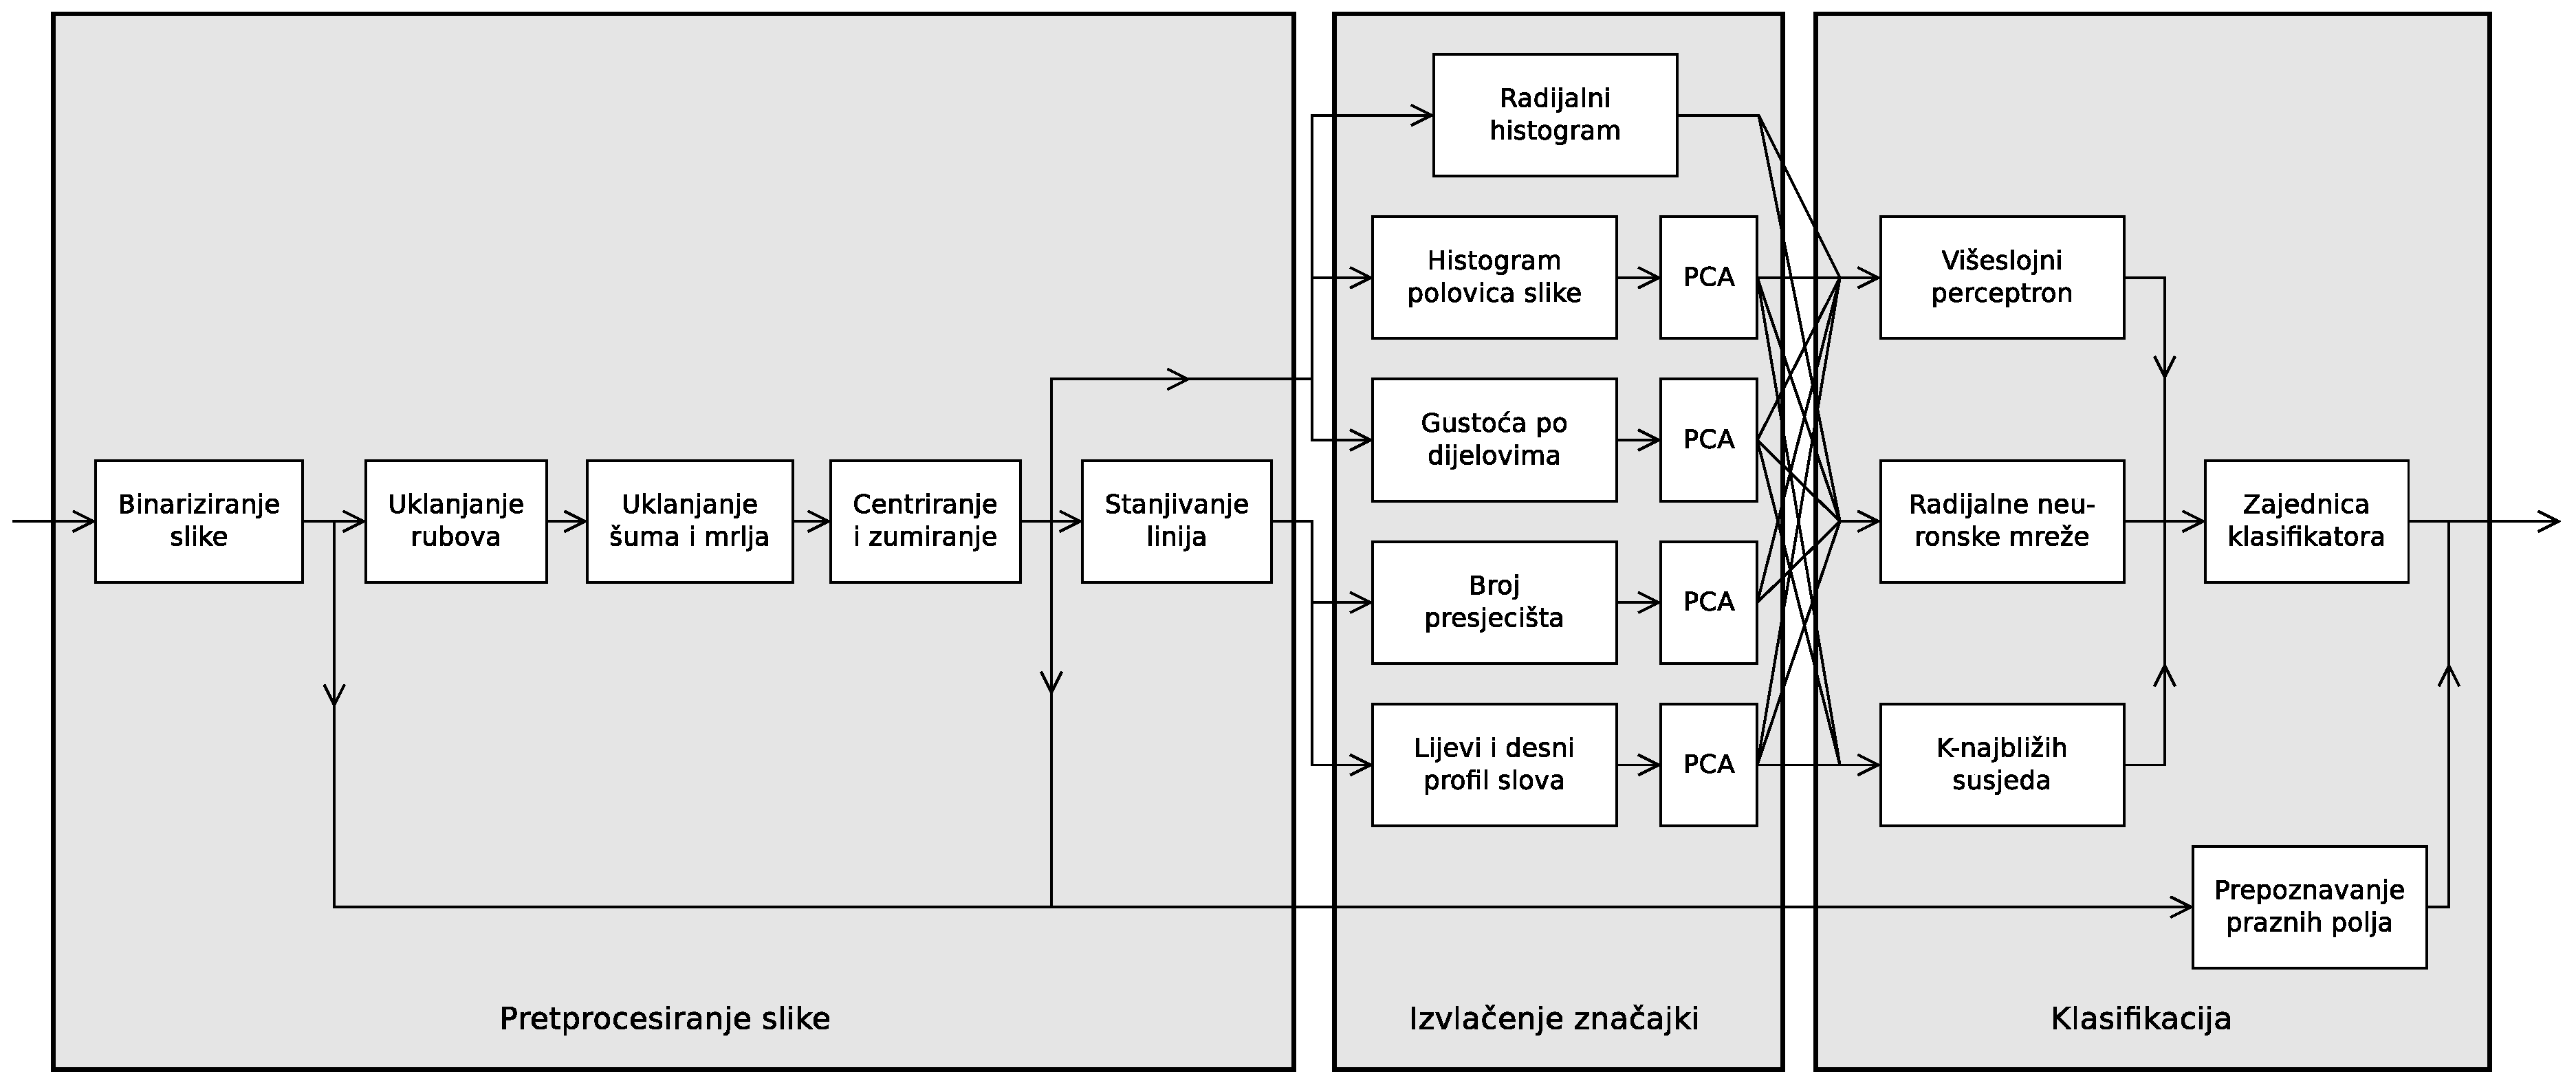
\includegraphics[width=\textwidth]{Diagram1.eps}
\caption{Prikaz podjele sustava}
\label{figure:cijeliSustav}
\end{figure*}

\section{Pretprocesiranje slike}
Prije izlučivanja značajki slova, potrebno je izvršiti pretprocesiranje slike.
Pretprocesiranje se sastoji od više koraka: binarizacije, uklanjanja rubova,
šuma i mrlja, centriranje i zumiranje slova te stanjivanja svih linija. S
obzirom na to da ispitni obrasci mogu biti skenirani različitim razlučivostima,
a slova mogu biti različitih veličina, debljina, intenziteta linija i pozicija u
polju, za precizno i kvalitetno izlučivanje značajki je potrebno svesti sva
slova na istu veličinu, debljinu i poziciju. Dobivene slike su identičnih
veličina (korištena je veličina 50x50), a slova su raširena preko cijele slike.

\subsection{Binariziranje slike}
Binariziranje slike pronalazi granični intenzitet (threshold), i onda sve
svijetlije slikovne elemente postavlja u bijelu boju, a sve tamnije u crnu.
Granični intenzitet je odabran tako da bar pola slike bude bijelo.

\subsection{Uklanjanje rubova}
Sličice skenirane iz obrazaca imaju u sebi i dio tamnih linija koje omeđuju
prostor za unos slova. Ove linije smetaju daljnjoj obradi, pa ih je potrebno ukloniti.
Rubovi se razlikuju od slike do slike, i nerijetko se preklapaju sa napisanim slovom.
Korišteni algoritam je rezultat dosta eksperimentiranja s raznim uzorcima, i
uzima u obzir profil boje ruba, njegovu širinu, te razne druge parametre.

Nakon binarizacije i uklanjanja rubova ispituje se je li slika prazna (opisano u potpoglavlju Prepoznavanje praznih polja) te ako jest, ona više ne
sudjeluje u daljnjem pretprocesiranju.

\subsection{Uklanjanje šuma i mrlja}
Uklanjanje šuma je izvedeno prema postupku koji su opisali K.\ Chinnasarn i
ostali \cite{chinnasarn2002removing} čime se u jednom prolazu znatno smanjuju
manje skupine crnih piksela na bijeloj, bijelih piksela na crnoj podlozi i
rubovi slova se zaglađuju. Postupak je primijenjen s parametrom $k = 5$.
Primijećeno je da se u rijetkim slučajevima pojavljuju artefakti, ali nisu imali
veći utjecaj na rezultate klasifikacije. Problem su stvarala i slova A koja, ako
su napisana debelom linijom, u nekim slučajevima gube bijelu površinu u sredini
slova.

Ponekad i nakon uklanjanja šumova ostaju razne skupine piksela koje nisu dio
slova. Drugi dio ovog filtra uklanja upravo takve mrlje (točke, crtice i slične
oblike koji su udaljeni od slova). Prvi korak algoritma je prepoznavanje
povezanih skupina piksela. Zatim se za najveću skupinu smatra da je glavni dio
slova. Nakon toga se gledaju udaljenosti između različitih skupina. Veće i
bliže skupine dijelovima slova smatraju se novim dijelom slova, a manje i dalje
skupine se smatraju mrljom i brišu se iz slike.

\subsection{Centriranje i zumiranje slova}
Ulazne slike je potrebno svesti na jedinstven i normiran oblik. Postupak 
centriranje slike pronalazi najmanji opisujući pravokutnik piksela slova  
i translatira ga u sredinu slike. Ovim postupak se osigurava invarijantnost
klasifikatora na translacije ulaznih slika. Postupak zumiranja skalira slova 
na određene dimenzije. Skaliranjem najmanjeg opisujećeg kvadrata, slovo se 
ne deformira i ne dolazi do gubitka informacija. Ovim postupkom se osigurava 
invarijantnost klasifikatora na skaliranje ulaznih slika.

\subsection{Stanjivanje linija}
Stanjivanje linija morfološka je operacija kojom se linije slova stanjuju na
debljinu jednog piksela. Time se postiže normalizirana debljina linija odnosno,
umanjuje se utjecaj stila pisanja na izgled slova. Implementiran algoritam
zasnovan je na algoritmu stanjivanja kakvog opisuje R.
Wang\cite{Wang2004Online}. Za svaki crni piksel, ispituje se njegovo susjedstvo
te određuje da li taj piksel treba ukloniti (obojati u bijelo) ili ne. Postupak
se ponavlja dokle god postoje pikseli koji zadovoljavaju uvjet uklanjanja.

\section{Izlučivanje značajki}
Kako bi klasifikacija bila što preciznija, napravljeno je više različitih načina
izlučivanja značajki. Svaka metoda ima svoje prednosti i nedostatke, a
korištenjem različitih metoda rezultati klasifikacije mogu biti znatno bolji
nego korištenjem samo jedne metode klasifikacije.

Većina korištenih metoda izlučivanja značajki vraća vrijednosti iz
visokodimenzionalnog prostora s kojim bi klasifikacija bila manje kvalitetna i
sporija. Zbog toga se koristi jedna od najčešćih metoda smanjivanja
dimenzionalnosti pomoću analize glavnih komponenti (engl.\ \emph{principal
component analysis}).

\subsection{Gustoća po dijelovima slike}
Izlučivanje značajki iz gustoće po dijelovima slike je najjednostavnija metoda
izlučivanja značajki. Slika se horizontalno i vertikalno dijeli na jednake
dijelove, a svakom dijelu se pridružuje realni broj od 0 do 1 koji predstavlja
odnos broja crnih i bijelih piksela. Broj 0 predstavlja da u tom dijelu nema
crnih piksela, a 1 predstavlja da nema bijelih piksela. U klasifikaciji je
podjela izvedena na 400 dijelova (20 horizontalnih i 20 vertikalnih), a
dimenzionalnost se smanjuje analizom glavnih komponenti na 20 dimenzija.

\subsection{Broj presjecišta}
Računamo koliko puta horizontalni i vertikalni pravci sijeku napisano slovo.
Za svaki redak slike krećemo se s lijeva na desno, i brojimo koliko puta
slikovni element mijenja boju iz bijele u crnu. To napravimo i za svaki stupac.
Za sliku 50x50, dobivamo 100 prirodnih brojeva koji dobro odražavaju oblik slova.

\subsection{Histogram polovica slike}
Slično kao i gustoća po dijelovima slike, histogram slike prikazuje odnos 
bijelih i crnih piksela na slici. Horizontalni histogram se računa na način 
da se za svaki piksel po horizontalnoj komponenti prebroji koliko ima crnih 
piksela u tom stupcu slike. Vertikalni histogram za svaki piksel po vertikalnoj 
komponenti, prebrojava koliko ima piksela u tom retku slike. Konkretna 
procedura izlučivanja značajki se sastoji od pronalaska 4 različita histograma: 
horizontalni histogram gornje polovice slike, horizontalni histogram donje 
polovice slike, vertikalni histogram lijeve polovice slike i vertikalni 
histogram desne polovice slike.

\subsection{Radijalni histogram}
Za potrebe računanja značajki radijalnog histograma, slika se promatra kao skup
točaka u polarnom koordinatnom sustavu a vrijednosti histograma su količine
crnih piksela koji se nalaze pojedinim intervalima kutova. Postupak se sastoji
od tri koraka a to su centriranje, određivanja kuta te kvantizacija kuta.
Centriranjem se svi pikseli translatiraju tako da se centroid (prosječna
pozicija) crnih piksela poklapa s ishodištem koordinatnog sustava. Iz
translatiranih koordinata u kartezijevom sustavu, računaju se koordinate u
polarnom sustavu, kut u odnosu na apscisu te udaljenost od ishodišta.
Kvantizacijom izračunatog kuta određuje se kojem intervalu kutova pojedini smjer
pripada.

\subsection{Profil slova}
Profil slova je broj piksela između opisujućeg pravokutnika (engl.
\emph{axis-aligned bounding box}) i ruba, tj. konture slova. Profil vrlo dobro
opisuje vanjski oblik slova. Računao se lijevi, desni, gornji i donji profil. Na
početku se određuje opisujući pravokutnik (svi pikseli slova su tada unutar
pravokutnika). Nakon toga slijedi određivanje broja piksela između opisujućeg
pravokutnika i gornjeg, desnog, donjeg i lijevog ruba slova.

\subsection{Huovi invarijantni momenti}
Neka je S skup svih piksela koji pripadaju slovu, i neka ih ima n.
Težište slova definiramo kao u \ref{equation:hu1}.
\begin{equation}
\overline{x} = \frac{1}{n}\displaystyle\sum_{x \in S}x
\overline{y} = \frac{1}{n}\displaystyle\sum_{y \in S}y
\label{equation:hu1}
\end{equation}

Sada definiramo centralni moment reda p+q preko \ref{equation:hu2}.
\begin{equation}
u(p,q) = \displaystyle\sum_{(x,y) \in S}(x-\overline{x})^p(y-\overline{y})^q
\label{equation:hu2}
\end{equation}

Korištenjem centralnih momenata mogu se izvesti izrazi čija vrijednost ne ovisi
o translaciji, rotaciji i veličini promatranog lika. Ti izrazi zovu se Huovi
invarijantni momenti i probali smo ih koristiti za izvlačenje značajki slova.
Algoritam je pokretan i prije i poslije stanjivanja linija, ali rezultati nisu
bili zadovoljavajući, pa je izbačen iz konačnog rješenja.


\section{Klasifikacija}
Svi klasifikatori su izrađeni tako da implementiraju sučelje koje ima tri metode
- klasifikaciju, učitavanje iz datoteke i pohranu u datoteku. Metoda
klasifikacije prima niz realnih brojeva koji predstavlja izlučene značajke, a
vraća polje u kojem su pohranjene vjerojatnosti klasifikacije odgovarajućeg
znaka. Klasifikator koji predstavlja zajednicu klasifikatora je odvojen od
drugih i ima vlastito sučelje. Jedna metoda prima sliku, a vraća vjerojatnosti
po znakovima. Druga metoda provjerava može li se vjerovati dobivenom rezultatu.

\subsection{Prepoznavanje praznih polja}
Za svaku sliku gleda se udio bijelih piksela te ako taj udio prijeđe prag od 0.995, slika se klasificira kao prazna.

\subsection{Višeslojni perceptron}
Višeslojni perceptron \cite{rosenblatt1958perceptron} (engl. \emph{multilayer
perceptron}) je vrsta neuronskih mreža koje imaju jedan ulazni, jedan izlazni i
jedan ili više skrivenih slojeva
\begin{equation}
y_i = \frac{1}{1 + \exp(v_i)}
\label{equation:sig}
\end{equation}

Za aktivacijsku funkciju je korištena funkcija \ref{equation:sig} (sigmoidna
funkcija) gdje je $v_i$ ulaz u aktivacijsku funkciju, a $y_i$ izlaz neurona. U
svim korištenim klasifikatorima izvedenih pomoću višeslojnog perceptrona broj
neurona u ulaznom sloju je 20 neurona te je korišten jedan skriveni sloj s 10
neurona. Treniranje je obavljeno s programskim paketom MATLAB pomoću povratne
propagacije pogreške \cite{rumelhart1986learning}. Tako istrenirane težine
neurona se učitavaju pri izradi objekta klasifikatora.

\subsection{Radijalne neuronske mreže}
Radijalne neuronske mreže sastoje se od tri sloja - ulaznog, skrivenog i
izlaznog sloja. Kod upotrebe ove vrste mreže, problemi klasifikacije uzoraka
rješavaju se nelinearnom transformacijom ulaznih uzoraka u prostor više
dimenzije od ulaznog prostora. U skrivenom se sloju koristi nelinearna skrivena
funkcija, dok se u izlaznom sloju koristi linearna funkcija.

\begin{equation}
\exp(-\left (b \left \| x - x_{i} \right \|  \right )^{2})
\label{equation:fZaUcenje}
\end{equation}

Za učenje u sklopu ovog projekta korištena je skrivena funkcija
\ref{equation:fZaUcenje}. Parametri ove skrivene funkcije su prag b te euklidska
udaljenost (norma) između pojedinog ulaznog uzorka i centra. Centri se biraju
između uzoraka iz skupa za učenje i fiksni su. Učenje je izvedeno uz pomoć
programskog paketa MATLAB. Potrebni parametri (kao što su broj skrivenih
neurona, željena pogreška te parametar širine određeni su eksperimentalno).
Korišteni su različiti parametri za  različite metode izlučivanja značajki
(parametar širine između 0.6 i 0.8 te različit broj skrivenih neurona, od 250 do
450). Dobivene vrijednosti težina učitavaju se iz datoteke pri izradi objekta
klasifikatora. Rezultati su navedeni u petom poglavlju Rezultati.

\subsection{Rekurzivne mreže}
Prilikom implementacije pokušalo se izgraditi rekurzivnu mrežu kao klasifikator slova. 
Zbog problema u fazi pamćenja rekurzivne mreže, tj. zbog pojave nestabilnih stanja, 
razvoj je prekinut i rekurzivna mreža nije upotrebljena u konačnom klasifikatoru.

\subsection{K-najbližih susjeda}
K-najbližih susjeda je jedna od najjednostavnijih metoda strojnog učenja. 
Klasifikator uspoređuje ulazni uzorak sa svim uzorcima iz skupa za učenje, 
u vektorskom prostoru značajki. Klasifikator pronalazi K sličnijih/najbližih 
uzoraka iz skupa za učenje. Vjerojatnost da ulazni uzorak pripada određenom 
razredu se računa kao broj uzoraka tog razredu među najbližih K, dijeljeno s K. 
Empirijski pronađeni najbolji K iznosi 4.

\subsection{Zajednica klasifikatora}
Kombiniranjem strojno naučenih algoritama može se povećati točnost
klasifikacije \cite{alpaydin2004introduction}. Varijacija između algoritama se
može postići različitim algoritmima, parametrima istog algoritma, različitim
modalitetima ulaza ili različitim skupovima za učenje. U ovoj aplikaciji je
varijacija postignuta različitim algoritmima i različitim modalitetima ulaza.
Sinergija je postignuta metodom jednostavnog glasanja, a ukupni rezultati su
skalirani tako da suma rezultata za sva slova bude 1. Isprobano je nekoliko
drugih metoda, ali se nisu pokazale bolje.

\section{Rezultati}
U aplikaciji je korišteno 48 ispunjenih i jedan neispunjen ispitni obrazac koji
su skenirani rezolucijama 200 dpi i 300 dpi. Neka slova su namjerno napisana
izrazito neuredno i nečitko kako bi bilo moguće provjeriti kako se aplikacija
ponaša na takvim uzrocima. Potrebno je napomenuti kako se u praktičnim uvjetima
ne očekuje da će se na ulaz aplikacije davati izrazito nečitka slova. Ovim
postupkom je dobiveno ukupno 5864 slike slova koje su korištene za klasifikaciju
(skup S). Za skup za učenje (skup U) i testiranje (skup T) su korištene slike
skenirane višim rezolucijama bez slova koja su jako loše napisana. Također,
u ta dva skupa se ne koriste prazna polja jer se takva slova klasificiraju
posebnim klasifikatorom. Skup za učenje čini slučajno odabranih 80\% tog
podskupa slova, ali tako da udio svih slova ostane jednak. U Tablici
\ref{table:brojSlova} je prikazan broj slova po skupovima.

\begin{table}[htb]
\centering
\begin{tabular}{lrrr} \toprule
Slovo & T & U+T & S \\ \midrule
prazno & 0 & 0 & 144 \\
- & 78 & 391 & 796 \\
A & 60 & 303 & 622 \\
B & 51 & 256 & 532 \\
C & 49 & 247 & 505 \\
D & 46 & 230 & 467 \\
E & 46 & 234 & 492 \\
F & 46 & 234 & 488 \\
G & 44 & 222 & 462 \\
H & 43 & 215 & 460 \\
I & 42 & 212 & 437 \\
J & 44 & 221 & 459 \\ \midrule
Ukupno & 549 & 2.765 & 5.864 \\ \bottomrule
\end{tabular}
\caption{Broj slova po skupovima}
\label{table:brojSlova}
\end{table}

U aplikaciji je korišteno ukupno 13 klasifikatora koji čine različite
kombinacije izlučenih značajki slike i klasifikatora. U Tablici
\ref{table:rezPoKlasif} se mogu vidjeti rezultati prema svim korištenim
klasifikatorima. Uzorak je klasificiran na način da je odabran onaj razred s
najvećom vjerojatnošću. Najbolje rezultate pokazuju radijalne neuronske mreže, a
svi korišteni klasifikatori imaju točnost veću od oko 85\%. Ovi rezultati se
odnose na skup za testiranje. Zadnji red prikazuje rezultat za zajednicu
klasifikatora i može se primijetiti kako sinergija svih klasifikatora daje
znatno bolje rezultate od bilo kojeg pojedinačnog klasifikatora. Iz toga se može
zaključiti kako su različite metode izlučivanja značajki dovoljno nekorelirane
pa se njihovim kombiniranjem dolazi do znatno boljih rezultata.

\begin{table}[htb]
\centering
\begin{tabular}{llr} \toprule
Klasifikator & Značajke & Točnost \\
\midrule
\multirow{5}{2cm}{Višeslojni perceptron}
 & Presjecišta & 86,70\% \\
 & Gustoća & 88,34\% \\
 & Histogram & 84,88\% \\
 & Profili & 88,89\% \\
 & Radijalni hist. & 88,52\% \\
\midrule
\multirow{5}{2cm}{Radijalne neuronske mreže}
 & Presjecišta & 87,25\% \\
 & Gustoća & 93,99\% \\
 & Histogram & 92,90\% \\
 & Profili slova & 94,54\% \\
 & Radijalni hist. & 93,26\% \\
\midrule
\multirow{3}{2cm}{K-najbližih susjeda}
 & Histogram & 88,16\% \\
 & Gustoća & 90,89\% \\
 & Profili & 88,53\% \\
\midrule
\multirow{1}{2cm}{Zajednica}
 & Sve & 97,45\% \\
\bottomrule
\end{tabular}
\caption{Broj slova po skupovima}
\label{table:rezPoKlasif}
\end{table}

Rezultati za zajednicu klasifikatora po ostalim skupovima uzoraka se može
vidjeti u Tablici \ref{table:rezultati}. Očekivano je kako najveću točnost ima
skup koji uključuje uzorke za učenje i testiranje.

\begin{table}[htb]
\centering
\begin{tabular}{lrrr} \toprule
 & T & U+T & S \\ \midrule
Ispravno & 535 & 2.739 & 5.715 \\
Neispravno & 14 & 26 & 149 \\
Točnost & 97,45\% & 99,06\% & 97,46\% \\ \bottomrule
\end{tabular}
\caption{Klasifikacija bez korištenja nesigurnosti}
\label{table:rezultati}
\end{table}

S obzirom na to da je jedan od zahtjeva aplikacije što je moguća manja pogreška
čak pod cijenu ručnog klasificiranja dijela uzoraka, određena je metoda
kako se neki rezultat smatra sigurnim ili nesigurnim. Rezultat se smatra
sigurnim ako je vjerojatnost najvjerojatnijeg slova veća od 53\% ili omjer dva
najvjerojatnija slova veća od 1,75. Ako se na ovaj način izvede klasifikacija,
dodatno se podiže točnost klasifikacije na 99,41\%. Rezultati za sve korištene
skupove uzoraka prikazani su u Tablici \ref{table:rezultati2}.

\begin{table}[htb]
\centering
\begin{tabular}{lrrr} \toprule
 & T & U+T & S \\ \midrule
Ispravno & 508 & 2678 & 5.533 \\
Neispravno & 3 & 4 & 51 \\
Nesigurno & 38 & 83 & 280 \\
Udio nesigurnih & 6,92\% & 3,00\% & 4,77\% \\
Točnost sigurnih & 99,41\% & 99,85\% & 99,09\% \\ \bottomrule
\end{tabular}
\caption{Klasifikacija s korištenjem nesigurnosti}
\label{table:rezultati2}
\end{table}

Dodatno podizanje točnosti klasifikacije se može postići tako da se prilikom
klasifikacije definira koja slova se očekuju kao rezultat. Primjerice, ako neki
ispitni obrasci imaju definirane odgovore od A do F, što je jedna od najčešće
korištenog broja odgovora, tada nije potrebno određivati vjerojatnosti slova od
G do J. U aplikaciji je to izvedeno kao ograničavanje izlazne dimenzionalnosti.
Prva dimenzija određuje vjerojatnost za prazno polje, druga za crticu, a od
treće do dvanaeste za slova od A do J. Na Slici \ref{figure:rezPoDim} je
prikazana točnost klasifikacije po broju dimenzija. Na gornjoj slici je
klasifikacija bez korištenja nesigurnosti, a na donjoj slici s korištenjem
nesigurnosti. Iz grafa se može potvrditi da ako se koriste odgovori od A do F,
tada je dimenzionalnost 8, a točnost klasifikacije uz korištenje nesigurnosti je
99,72\%.

\begin{figure}
\centering
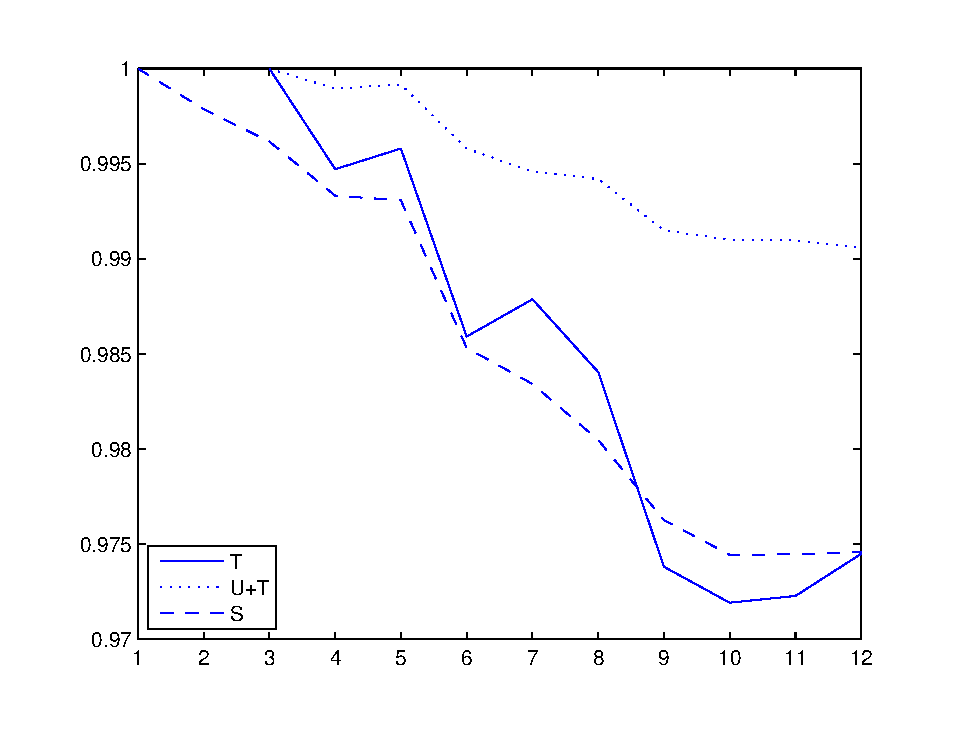
\includegraphics[scale=0.5]{accByDim1.eps}
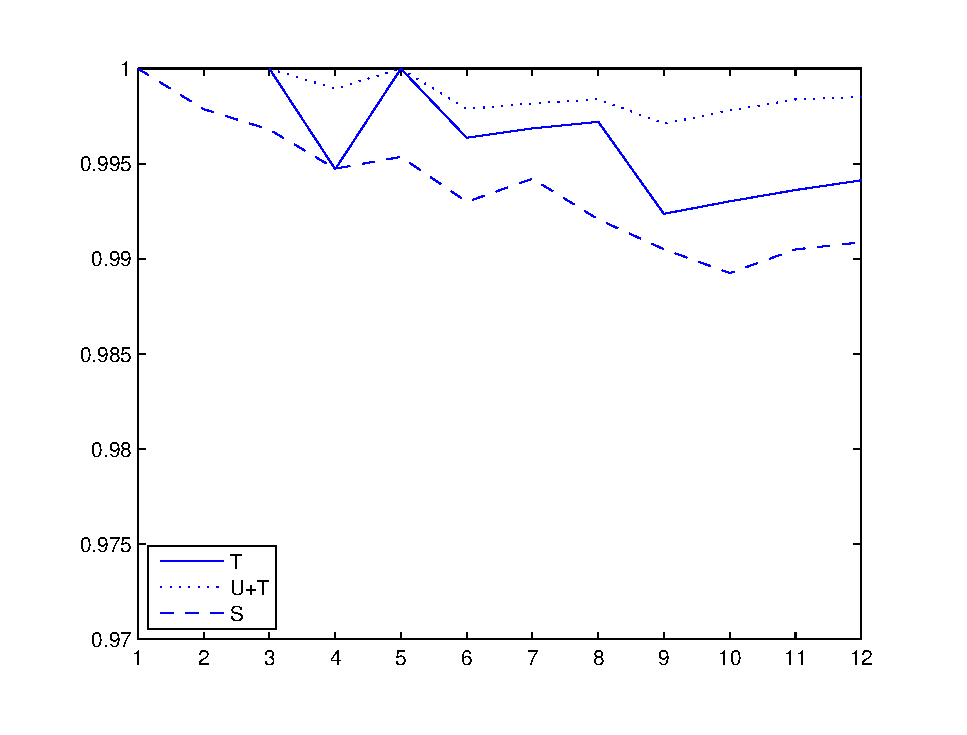
\includegraphics[scale=0.5]{accByDim2.eps}
\caption{Točnost klasifikacije po broju dimenzija bez upotrebe nesigurnosti
(gornja slika) i s upotrebom nesigurnosti (donja slika)}
\label{figure:rezPoDim}
\end{figure}

Na Slici \ref{figure:rezPoBrojuKlas} je prikazana točnost klasifikacije prema
broju korištenih klasifikatora. Iz grafa se može zaključiti kako dodavanjem
novih metoda izvlačenja značajki slike, klasifikatora i sličnog ne može znatno
povisiti udio ispravnih klasifikacija.

\begin{figure}
\centering
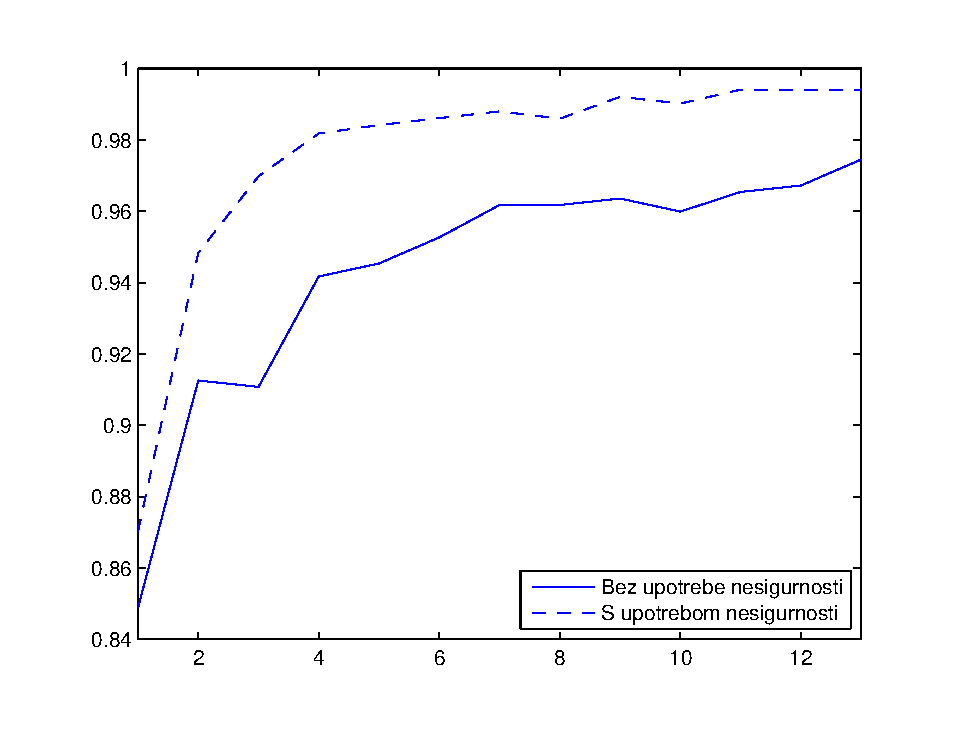
\includegraphics[scale=0.5]{accByClassifCount.eps}
\caption{Točnost klasifikacije po broju klasifikatora}
\label{figure:rezPoBrojuKlas}
\end{figure}


\section{Zaključak}
U ovom radu implementirano je nadzirano učenje nad rukom pisanim odgovorima na
ispitnim obrascima. Testirano je šest metoda izlučivanja značajki i četiri
različita klasifikatora. Od isprobanih metoda izlučivanja značajki uspješnim
su se pokazali gustoća po dijelovima slike, broj horizontalnih presjecišta,
histogrami polovica slika, radijalni histogram i profili slova, a samo Huovi
invarijantni momenti su se pokazali nedovoljno točnim. Od klasifikatora
najboljim su se pokazale radijalne neuronske mreže, dovoljno dobrim višeslojni
perceptron i K-najbližih susjeda, a razvoj rekurzivnih mreža je zbog većeg broja
nestabilnih stanja prekinut. Ipak, sinergijom raznih kombinacija izlučivanja
značajki i metoda klasifikacije pomoću jednostavnog glasanja ostvarena je
sinergija klasifikatora. Time se pokazalo da su ovakva izlučivanja značajki
dovoljno nekorelirana. Pokazano je i kako se analizom glavnih komponenti može
uspješno smanjiti dimenzionalnost bez većeg gubitka korisnih informacija.

Nastavak rada se treba orijentirati na povećanje točnosti i brzine rada krajnje
klasifikacije. Povećanje točnosti se najvjerojatnije može postići većim skupom
uzoraka, dodavanjem novih metoda klasifikacije (primjerice, u ovom radu nije
korištena jedna od najpopularnijih metoda klasifikacije - stroj s potpornim
vektorima), dodatnim elementima pretprocesiranja (primjerice, ispravljanje
nagiba) i naprednijim metodama kombinacije strojno naučenih algoritama. Moguće
je izraditi više binarnih klasifikatora, a rezultat dobiti preko izlaznog koda s
ispravljanjem pogreške.

Brzina je zadovoljavajuća za trenutačan problem jer brzo
prepoznaje prazna polja, a dodatna brzina se može postići optimiziranjem
postojećih komponenti i drugačijim ujedinjavanjem rezultata klasifikatora
(primjerice, pomoću boostanja).

% Bibliografija
\bibliographystyle{amsplain}
\bibliography{literatura}

\end{document}
